\PassOptionsToPackage{unicode}{hyperref}
\documentclass[aspectratio=1610, 11pt]{beamer}

\usepackage{amsmath}
\usepackage{amssymb}
\usetheme{tudo}

\title{Datenstrukturen, Algorithmen und Prorammierung~2}
\author[A.~Coja-Oghlan]{Amin Coja-Oghlan}
\institute[DAP2]{Lehrstuhl Informatik 2\\Fakult\"at f\"ur Informatik}

\renewcommand{\vec}[1]{\boldsymbol{#1}}
\newcommand\NULL{{\tt NULL}}
\newcommand\dd{\mathrm d}
\newcommand\eul{\mathrm e}
\newcommand\cA{\mathcal A}
\newcommand\cB{\mathcal B}
\newcommand\cC{\mathcal C}
\newcommand\cD{\mathcal D}
\newcommand\cE{\mathcal E}
\newcommand\cF{\mathcal F}
\newcommand\cG{\mathcal G}
\newcommand\cH{\mathcal H}
\newcommand\cI{\mathcal I}
\newcommand\cJ{\mathcal J}
\newcommand\cK{\mathcal K}
\newcommand\cL{\mathcal L}
\newcommand\cM{\mathcal M}
\newcommand\cN{\mathcal N}
\newcommand\cO{\mathcal O}
\newcommand\cP{\mathcal P}
\newcommand\cQ{\mathcal Q}
\newcommand\cR{\mathcal R}
\newcommand\cS{\mathcal S}
\newcommand\cT{\mathcal T}
\newcommand\cU{\mathcal U}
\newcommand\cV{\mathcal V}
\newcommand\cW{\mathcal W}
\newcommand\cX{\mathcal X}
\newcommand\cY{\mathcal Y}
\newcommand\cZ{\mathcal Z}
\newcommand\fA{\mathfrak A}
\newcommand\fB{\mathfrak B}
\newcommand\fC{\mathfrak C}
\newcommand\fD{\mathfrak D}
\newcommand\fE{\mathfrak E}
\newcommand\fF{\mathfrak F}
\newcommand\fG{\mathfrak G}
\newcommand\fH{\mathfrak H}
\newcommand\fI{\mathfrak I}
\newcommand\fJ{\mathfrak J}
\newcommand\fK{\mathfrak K}
\newcommand\fL{\mathfrak L}
\newcommand\fM{\mathfrak M}
\newcommand\fN{\mathfrak N}
\newcommand\fO{\mathfrak O}
\newcommand\fP{\mathfrak P}
\newcommand\fQ{\mathfrak Q}
\newcommand\fR{\mathfrak R}
\newcommand\fS{\mathfrak S}
\newcommand\fT{\mathfrak T}
\newcommand\fU{\mathfrak U}
\newcommand\fV{\mathfrak V}
\newcommand\fW{\mathfrak W}
\newcommand\fX{\mathfrak X}
\newcommand\fY{\mathfrak Y}
\newcommand\fZ{\mathfrak Z}
\newcommand\fa{\mathfrak a}
\newcommand\fb{\mathfrak b}
\newcommand\fc{\mathfrak c}
\newcommand\fd{\mathfrak d}
\newcommand\fe{\mathfrak e}
\newcommand\ff{\mathfrak f}
\newcommand\fg{\mathfrak g}
\newcommand\fh{\mathfrak h}
%\newcommand\fi{\mathfrak i}
\newcommand\fj{\mathfrak j}
\newcommand\fk{\mathfrak k}
\newcommand\fl{\mathfrak l}
\newcommand\fm{\mathfrak m}
\newcommand\fn{\mathfrak n}
\newcommand\fo{\mathfrak o}
\newcommand\fp{\mathfrak p}
\newcommand\fq{\mathfrak q}
\newcommand\fr{\mathfrak r}
\newcommand\fs{\mathfrak s}
\newcommand\ft{\mathfrak t}
\newcommand\fu{\mathfrak u}
\newcommand\fv{\mathfrak v}
\newcommand\fw{\mathfrak w}
\newcommand\fx{\mathfrak x}
\newcommand\fy{\mathfrak y}
\newcommand\fz{\mathfrak z}
\newcommand\vA{\vec A}
\newcommand\vB{\vec B}
\newcommand\vC{\vec C}
\newcommand\vD{\vec D}
\newcommand\vE{\vec E}
\newcommand\vF{\vec F}
\newcommand\vG{\vec G}
\newcommand\vH{\vec H}
\newcommand\vI{\vec I}
\newcommand\vJ{\vec J}
\newcommand\vK{\vec K}
\newcommand\vL{\vec L}
\newcommand\vM{\vec M}
\newcommand\vN{\vec N}
\newcommand\vO{\vec O}
\newcommand\vP{\vec P}
\newcommand\vQ{\vec Q}
\newcommand\vR{\vec R}
\newcommand\vS{\vec S}
\newcommand\vT{\vec T}
\newcommand\vU{\vec U}
\newcommand\vV{\vec V}
\newcommand\vW{\vec W}
\newcommand\vX{\vec X}
\newcommand\vY{\vec Y}
\newcommand\vZ{\vec Z}
\newcommand\va{\vec a}
\newcommand\vb{\vec b}
\newcommand\vc{\vec c}
\newcommand\vd{\vec d}
\newcommand\ve{\vec e}
\newcommand\vf{\vec f}
\newcommand\vg{\vec g}
\newcommand\vh{\vec h}
\newcommand\vi{\vec i}
\newcommand\vj{\vec j}
\newcommand\vk{\vec k}
\newcommand\vl{\vec l}
\newcommand\vm{\vec m}
\newcommand\vn{\vec n}
\newcommand\vo{\vec o}
\newcommand\vp{\vec p}
\newcommand\vq{\vec q}
\newcommand\vr{\vec r}
\newcommand\vs{\vec s}
\newcommand\vt{\vec t}
\newcommand\vu{\vec u}
\renewcommand\vv{\vec v}
\newcommand\vw{\vec w}
\newcommand\vx{\vec x}
\newcommand\vy{\vec y}
\newcommand\vz{\vec z}
\renewcommand\AA{\mathbb A}
\newcommand\NN{\mathbb N}
\newcommand\ZZ{\mathbb Z}
\newcommand\PP{\mathbb P}
\newcommand\QQ{\mathbb Q}
\newcommand\RR{\mathbb R}
\newcommand\RRpos{\mathbb R_{\geq0}}
\renewcommand\SS{\mathbb S}
\newcommand\CC{\mathbb C}
\newcommand{\ord}{\mathrm{ord}}
\newcommand{\id}{\mathrm{id}}
\newcommand{\pr}{\mathrm{P}}
\newcommand{\Vol}{\mathrm{vol}}
\newcommand\norm[1]{\left\|{#1}\right\|} 
\newcommand\sign{\mathrm{sign}}
\newcommand{\eps}{\varepsilon}
\newcommand{\abs}[1]{\left|#1\right|}
\newcommand\bc[1]{\left({#1}\right)} 
\newcommand\cbc[1]{\left\{{#1}\right\}} 
\newcommand\bcfr[2]{\bc{\frac{#1}{#2}}} 
\newcommand{\bck}[1]{\left\langle{#1}\right\rangle} 
\newcommand\brk[1]{\left\lbrack{#1}\right\rbrack} 
\newcommand\scal[2]{\bck{{#1},{#2}}} 
\newcommand{\vecone}{\mathbb{1}}
\newcommand{\tensor}{\otimes}
\newcommand{\diag}{\mathrm{diag}}
\newcommand{\ggt}{\mathrm{ggT}}
\newcommand{\kgv}{\mathrm{kgV}}
\newcommand{\trans}{\top}
\newcommand{\Karonski}{Karo\'nski}
\newcommand{\Erdos}{Erd\H{o}s}
\newcommand{\Renyi}{R\'enyi}
\newcommand{\Lovasz}{Lov\'asz}
\newcommand{\Juhasz}{Juh\'asz}
\newcommand{\Bollobas}{Bollob\'as}
\newcommand{\Furedi}{F\"uredi}
\newcommand{\Komlos}{Koml\'os}
\newcommand{\Luczak}{\L uczak}
\newcommand{\Kucera}{Ku\v{c}era}
\newcommand{\Szemeredi}{Szemer\'edi}

\newcommand{\mytitle}{Graphen}

\begin{document}

\frame[plain]{\titlepage}

\begin{frame}\frametitle{\mytitle}
	\begin{exampleblock}{Worum geht es?}
		\begin{itemize}
			\item Graphen sind ein Grundbaustein der Algorithmik
			\item \dots und der Diskreten Mathematik.
			\item Unz\"ahligen Anwendungen sind als Graphen modellierbar, z.B.
				\begin{itemize}
					\item ein Stra\ss en-- oder Schienennetz
					\item ein Kontaktnetzwerk
					\item Abh\"angigkeiten zwischen Prozessen
					\item der Verdrahtungsplan eines Chips
					\item das Gehirn
				\end{itemize}
			\item dabei treten dieselben grundlegenden Problemstellungen auf
			\item Graphenalgorithmen sind also extrem vielseitig einsetzbar
		\end{itemize}
	\end{exampleblock}
\end{frame}

%\begin{frame}\frametitle{\mytitle}
%	\begin{block}{Thema dieser Vorlesung}
%		\begin{itemize}
%			\item Grundbegriffe der Graphentheorie
%			\item Zusammenhang
%		\end{itemize}
%	\end{block}
%\end{frame}

\begin{frame}\frametitle{\mytitle}
	\hfill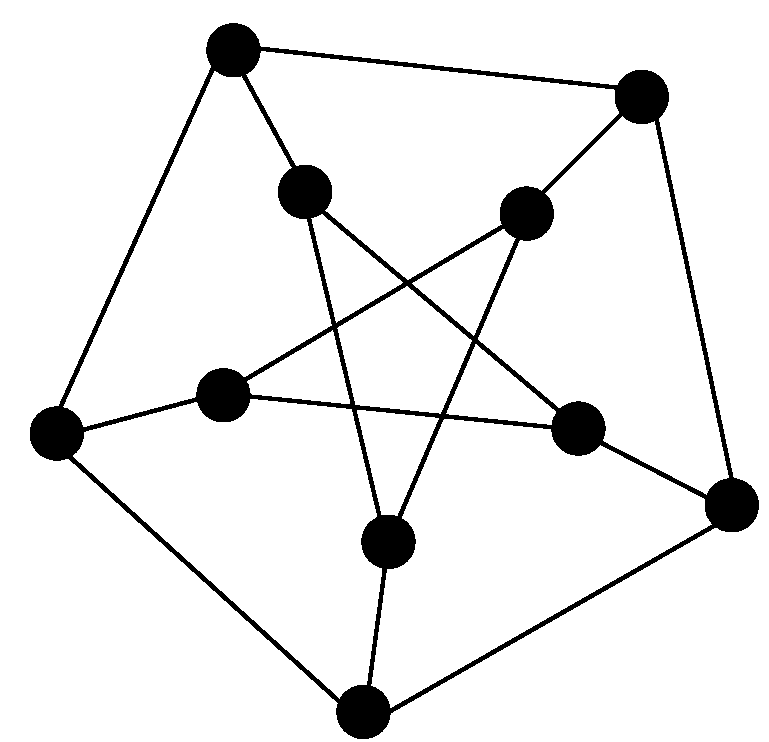
\includegraphics[height=20mm]{images/petersen2.pdf}
	\begin{block}{Definition}
		Ein \alert{Graph} $G=(V,E)$ besteht aus
		\begin{itemize}
			\item einer Menge $V$ von \alert{Knoten} und
			\item einer Menge $E$ von \alert{Kanten},
		\end{itemize}
		so da\ss\ jede Kante $e\in E$ eine zweielementige Teilmenge von $V$ ist.

		\medskip
		\itshape Graphisch stellen wir die Knoten als Punkte dar und die Kanten als ungerichtete Verbindungslinien.
	\end{block}
\end{frame}

\begin{frame}\frametitle{\mytitle}
	\begin{overprint}
		\onslide<1>
	\hfill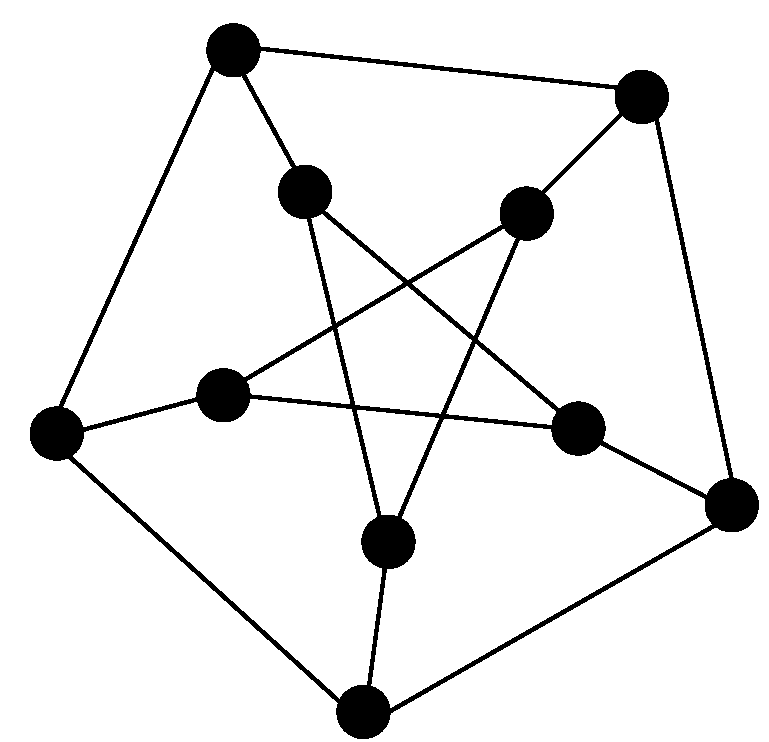
\includegraphics[height=40mm]{images/petersen2.pdf}
	\begin{exampleblock}{Beispiel: der Petersen-Graph}
		\begin{itemize}
			\item 10 Knoten
			\item 15 Kanten
		\end{itemize}
	\end{exampleblock}
		\onslide<2>
	\hfill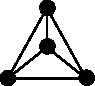
\includegraphics[height=20mm]{images/k4.pdf}
		\begin{exampleblock}{Beispiel: der vollst\"andige Graph $K_4$}
		\begin{itemize}
			\item 4 Knoten
			\item jeder der $\binom 42=6$ m\"oglichen Kanten ist vorhanden
		\end{itemize}
	\end{exampleblock}
		\onslide<3>
	\hfill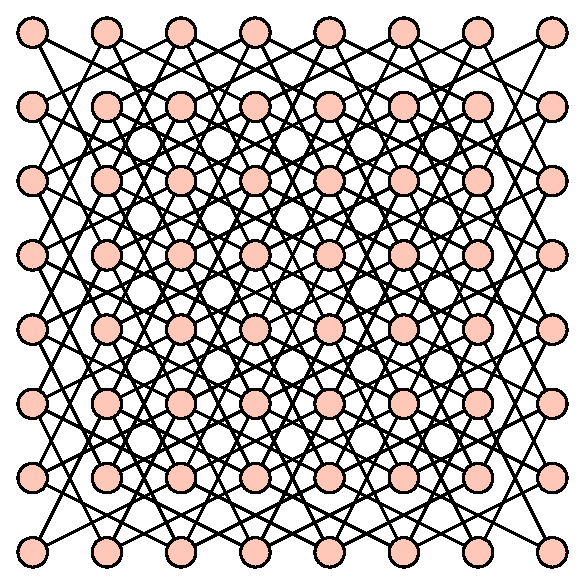
\includegraphics[height=40mm]{images/springergraph.pdf}
		\begin{exampleblock}{Beispiel: das Springerproblem}
		\begin{itemize}
			\item {\itshape Ist es m\"oglich, mit einem Springer alle 64 Felder eines Schachbrettes in einem Zug genau einmal zu besuchen?}
			\item Die Knoten entsprechen den Feldern, die Kanten den m\"oglichen Z\"ugen
		\end{itemize}
	\end{exampleblock}
		\onslide<4>
		\begin{exampleblock}{Konvention}
		\begin{itemize}
			\item angenommen $G=(V,E)$ ist ein Graph
			\item sofern nicht ausdr\"ucklich anders angegeben, nehmen wir stets an, da\ss\ die Knotenmenge endlich ist.
			\item mit $V(G)=V$ und $E(G)=E$ werden Knoten- und Kantenmenge eines Graphen bezeichnet.
			\item f\"ur eine Kante $\{u,v\}$ verwenden wir die Kurzschreibweise $uv$.
			\item per Definition enthalten Graphen keine \alert{Mehrfachkanten} und keine \alert{Schleifen}.
		\end{itemize}
	\end{exampleblock}
	\end{overprint}
\end{frame}

\begin{frame}\frametitle{\mytitle}
	\begin{overprint}
		\onslide<1>
	\hfill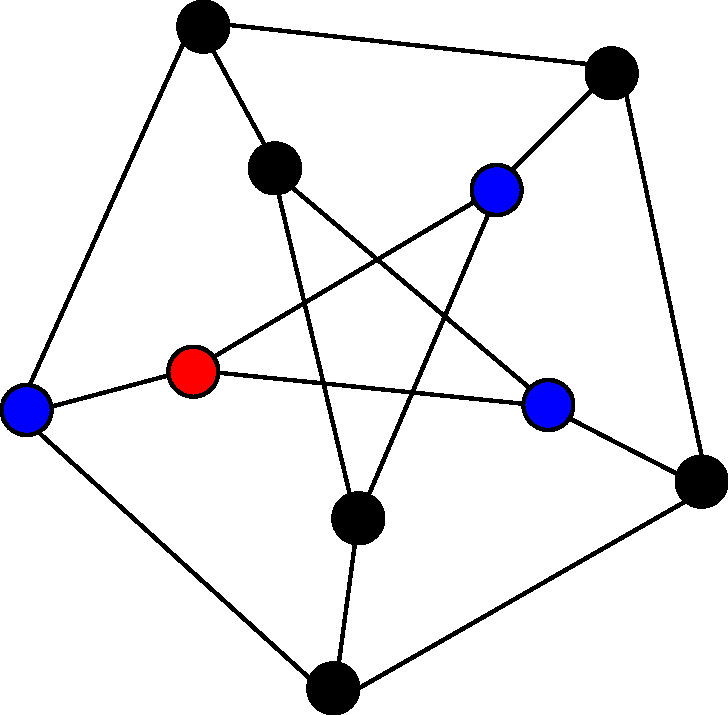
\includegraphics[height=25mm]{images/petersen4.pdf}
	\begin{block}{Definition}
		Angenommen $G=(V,E)$ ist ein Graph. 
		\begin{itemize}
			\item die \alert{Nachbarschaft} von $v\in V$ ist
				\begin{align*}
					\partial_Gv=\cbc{u\in V:uv\in E}.
				\end{align*}
			\item der \alert{Grad} von $v$ ist $d_G(v)=|\partial_Gv|$.
		\end{itemize}
	\end{block}
		\onslide<2>
	\hfill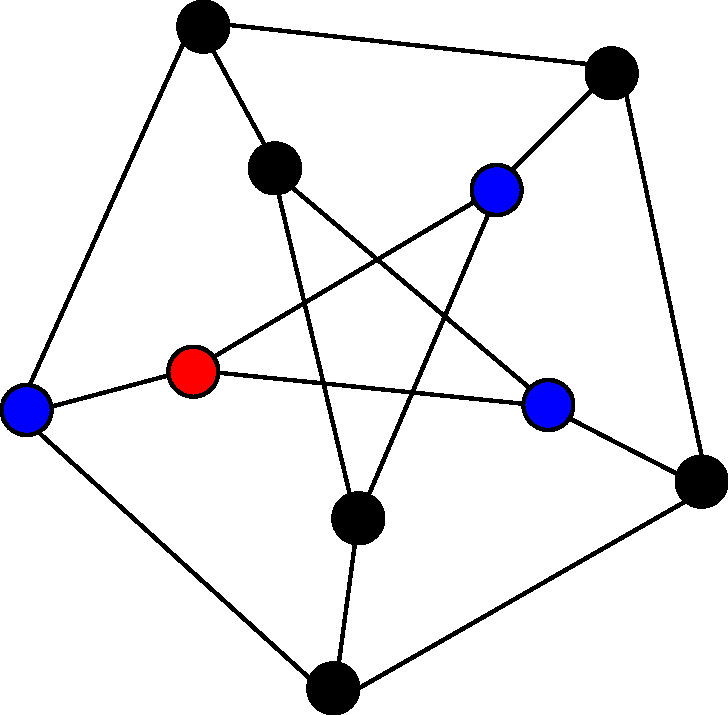
\includegraphics[height=25mm]{images/petersen4.pdf}
	\begin{block}{Definition}
		Angenommen $G=(V,E)$ ist ein Graph. 
		\begin{itemize}
			\item die Knoten $v,w\in V$ sind \alert{adjazent} oder \alert{benachbart}, falls $vw\in E$.
			\item der Knoten $v$ und die Kante $e\in E$ sind \alert{inzident}, falls $v\in e$.
		\end{itemize}
	\end{block}
		\onslide<3>
	\hfill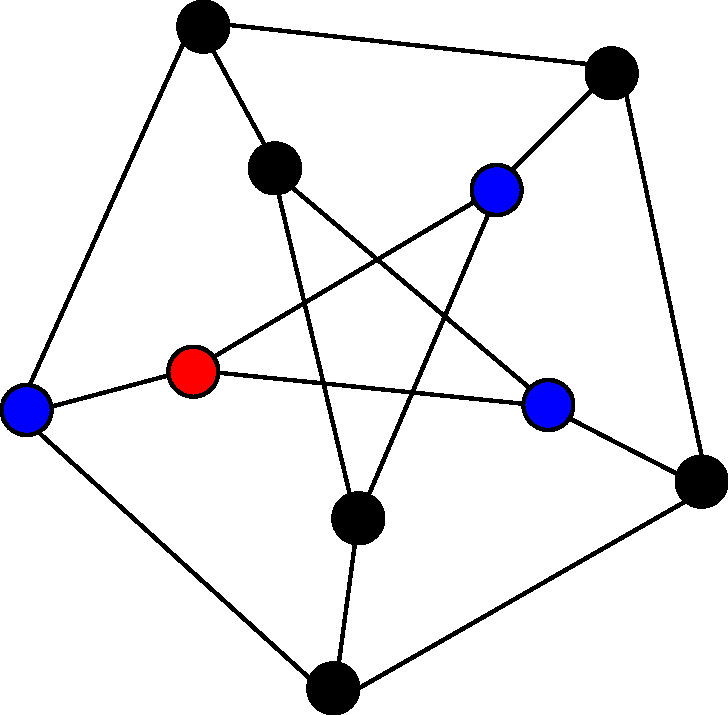
\includegraphics[height=25mm]{images/petersen4.pdf}
	\begin{block}{Definition}
		Angenommen $G=(V,E)$ ist ein Graph. 
		\begin{itemize}
			\item der \alert{Maximalgrad} von $G$ ist $\Delta(G)=\max_{v\in V}d_G(v).$
			\item der \alert{Minimalgrad} von $G$ ist $\delta(G)=\min_{v\in V}d_G(v).$
			\item der Graph ist \alert{$k$-regul\"ar}, falls $\Delta(G)=\delta(G)=k$.
		\end{itemize}
	\end{block}
		\onslide<4>
	\hfill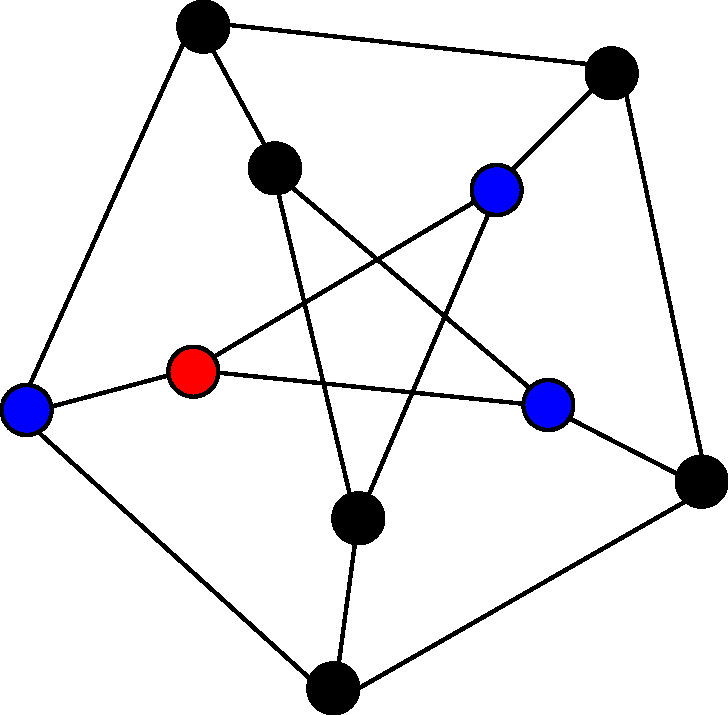
\includegraphics[height=25mm]{images/petersen4.pdf}
	\begin{block}{Definition}
		Angenommen $G=(V,E)$ ist ein Graph. Das \alert{Komplement} $\bar G$ von $G$ ist der Graph mit Knotenmenge $V(\bar G)=V$ und Kantenmenge
		\begin{align*}
			E(\bar G)=\cbc{uv:u,v\in V,\,u\neq v,\,uv\not\in E}.
		\end{align*}
	\end{block}
	\end{overprint}
\end{frame}

\begin{frame}\frametitle{\mytitle}
	\begin{overprint}
		\onslide<1>
	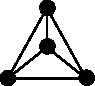
\includegraphics[height=20mm]{images/k4.pdf}\hfill
\includegraphics[height=20mm]{images/e4.pdf}
	\begin{exampleblock}{Beispiel: der vollst\"andige und der leere Graph}
		\begin{itemize}
			\item sei $\ell\geq1$.
			\item mit $K_\ell$ wird der \alert{vollst\"andige Graph} auf $\ell$ Knoten bezeichnet:
				\begin{align*}
					V(K_\ell)&=\cbc{1,2,\ldots,\ell}&
					E(K_\ell)&=\cbc{vw:1\leq v<w\leq\ell}
				\end{align*}
			\item das Komplement $\bar K_\ell$ ist der \alert{leere Graph}.
		\end{itemize}
	\end{exampleblock}
		\onslide<2>
	\hfill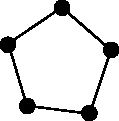
\includegraphics[height=30mm]{images/c5.pdf}
	\begin{exampleblock}{Beispiel: Kreise}
		\begin{itemize}
			\item sei $\ell\geq1$.
			\item mit $C_\ell$ wird der \alert{Kreis} auf $\ell$ Knoten bezeichnet:
				\begin{align*}
					V(C_\ell)&=\cbc{1,2,\ldots,\ell}\\
					E(C_\ell)&=\cbc{\cbc{1,2},\cbc{2,3},\cbc{3,4},\ldots,\cbc{\ell,1}}
				\end{align*}
		\end{itemize}
	\end{exampleblock}
		\onslide<3>
	\hfill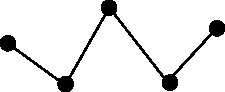
\includegraphics[height=30mm]{images/p5.pdf}
	\begin{exampleblock}{Beispiel: Pfade}
		\begin{itemize}
			\item sei $\ell\geq1$.
			\item mit $P_\ell$ wird der \alert{Pfad} auf $\ell$ Knoten bezeichnet:
				\begin{align*}
					V(P_\ell)&=\cbc{1,2,\ldots,\ell}\\
					E(P_\ell)&=\cbc{\cbc{1,2},\cbc{2,3},\cbc{3,4},\ldots,\cbc{\ell-1,\ell}}
				\end{align*}
		\end{itemize}
	\end{exampleblock}
	\end{overprint}
\end{frame}
 
\begin{frame}\frametitle{\mytitle}
	\begin{overprint}
		\onslide<1>
\begin{block}{Lemma}
		F\"ur einen Graphen $G$ gilt stets $\displaystyle\sum_{v\in V(G)}d_G(v)=2|E(G)|.$
	\end{block}
	\onslide<2>
\begin{exampleblock}{Beweis}
	\begin{itemize}
		\item Wir f\"uhren Induktion nach der Anzahl der Kanten.
		\item In einem leeren Graphen haben wir
			$$\sum_{v\in V(G)}d_G(v)=0=|E(G)|.$$
		\item Wenn wir jetzt $G$ aus $G'$ erhalten, indem wir eine Kanten hinzuf\"ugen, dann gilt nach Induktion
			\begin{align*}
				\sum_{v\in V(G)}d_G(v)&=2+\sum_{v\in V(G')}d_{G'}(v)=2+2|E(G')|=2|E(G)|.
			\end{align*}
	\end{itemize}
	\end{exampleblock}
	\end{overprint}
\end{frame}

\begin{frame}\frametitle{\mytitle}
	\begin{overprint}
		\onslide<1>
	\begin{block}{Definition}
		Zwei Graphen $G=(V,E)$ und $G'=(V',E')$ sind \emph{isomorph}, wenn es eine bijektive Abbildung $\phi:V\to V'$ gibt, so da\ss
		\begin{align*}
			vw&\in E&\Leftrightarrow&&\phi(v)\phi(w)\in E'&&\mbox{f\"ur alle }v,w\in V.
		\end{align*}
	\end{block}
	\end{overprint}
\end{frame}

\begin{frame}\frametitle{\mytitle}
	\begin{overprint}
		\onslide<1>
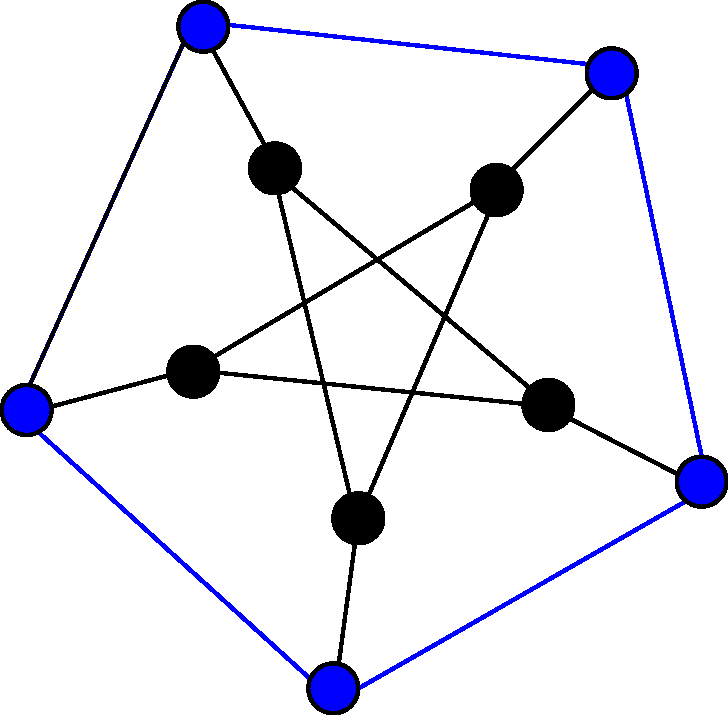
\includegraphics[height=30mm]{images/subgraphNonInduced.pdf}\hfill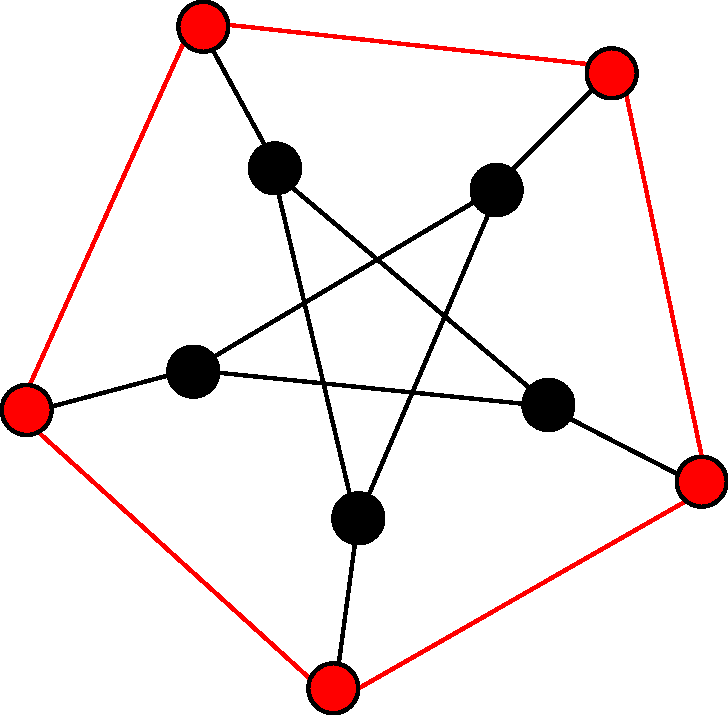
\includegraphics[height=30mm]{images/subgraph.pdf}
	\begin{block}{Definition}
		Ein Graph $G=(V,E)$ enth\"alt einen Graphen $G'=(V',E')$
		\begin{itemize}
			\item als \alert{Untergraph}, falls $V'\subseteq V$ und $E'\subseteq E$.
			\item als \alert{induzierten Untergraphen}, falls $V'\subseteq V$ und $E'=\cbc{vw:v,w\in V',\,vw\in E}.$
		\end{itemize}
	\end{block}
	\end{overprint}
\end{frame}

\begin{frame}\frametitle{\mytitle}
	\begin{overprint}
		\onslide<1>
\hfill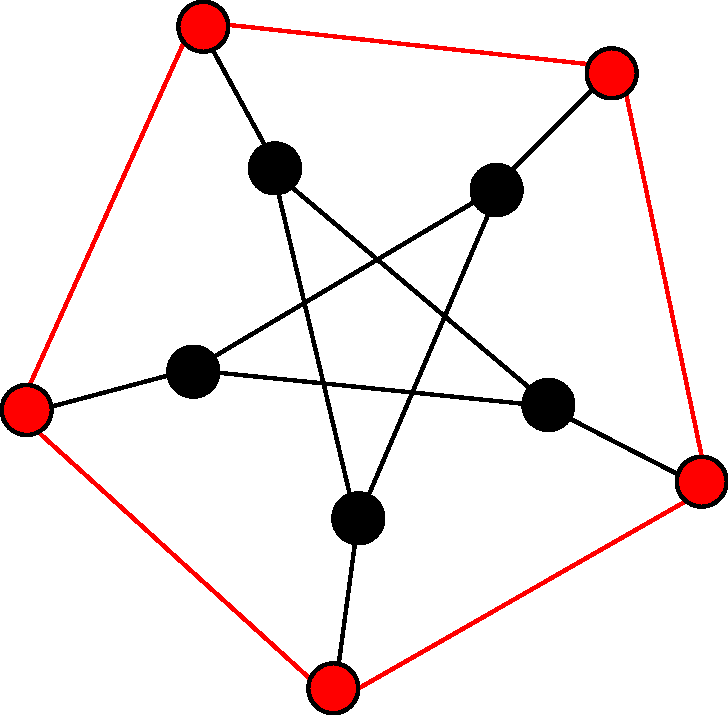
\includegraphics[height=30mm]{images/subgraph.pdf}
	\begin{block}{Definition}
		Der von $G=(V,E)$ auf $S\subseteq V$ \alert{induzierte Untergraph} ist der Graph $G[S]=(S,E(G[S]))$ mit Kantenmenge
				\begin{align*}
					E(G[S])=\cbc{vw:v,w\in S,\,vw\in E}.
				\end{align*}
	\end{block}
	\end{overprint}
\end{frame}

\begin{frame}\frametitle{\mytitle}
	\begin{overprint}
		\onslide<1>
	\begin{exampleblock}{L\"oschen von Knoten und Kanten}
		Angenommen $G=(V,E)$ ist ein Graph.
		\begin{itemize}
			\item Wenn $U\subseteq V$ eine Menge von Knoten ist, definiere $G-U=G[V\setminus U].$
			\item Wenn $F\subseteq E$ eine Menge von Kanten ist, definiere $G-F=(V,E\setminus F).$
		\end{itemize}
	\end{exampleblock}
	\end{overprint}
\end{frame}

\begin{frame}\frametitle{\mytitle}
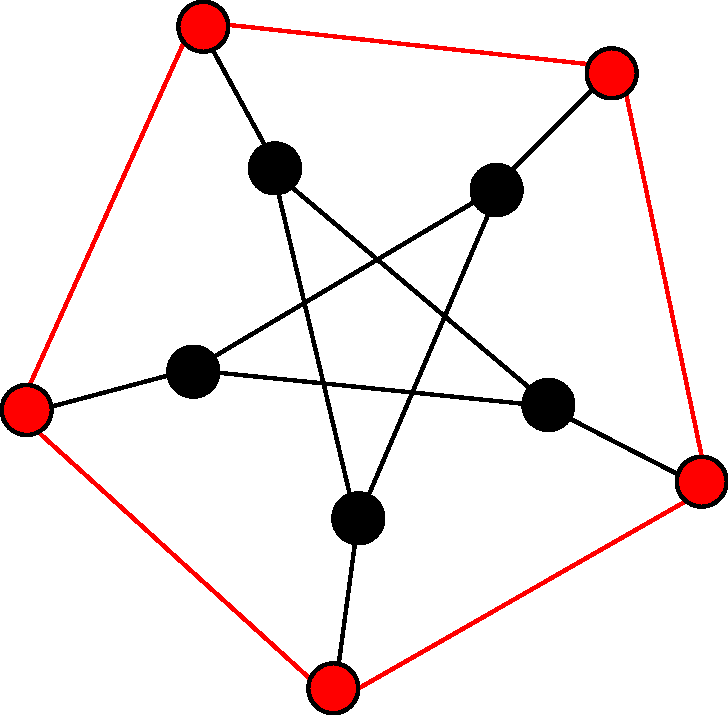
\includegraphics[height=20mm]{images/subgraph.pdf}\hfill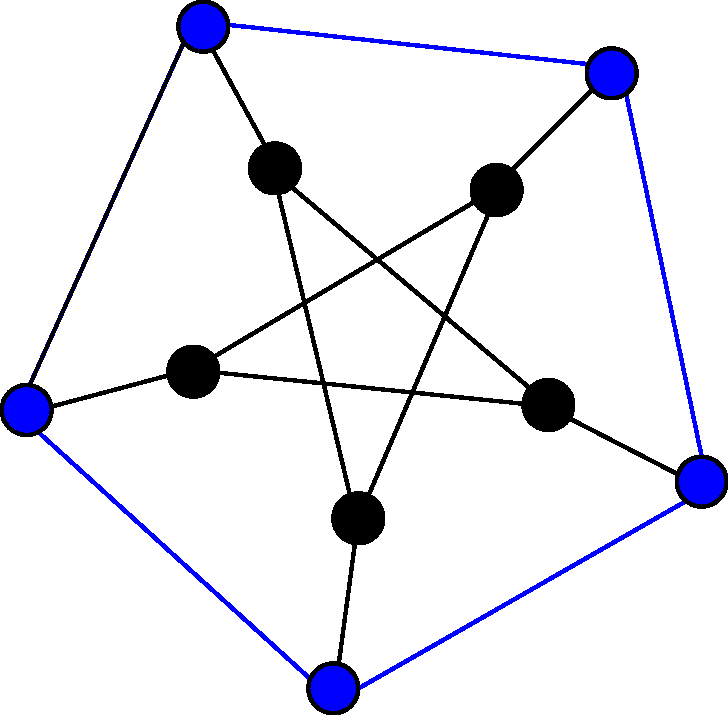
\includegraphics[height=20mm]{images/subgraphNonInduced.pdf}
	\begin{overprint}
		\onslide<1>
	\begin{block}{Definition}
		Ein Graph $G=(V,E)$ enth\"alt
		\begin{itemize}
			\item eine \alert{induzierte Kopie} eines Graph $G'=(V',E')$, wenn es eine Menge $S\subseteq V$ gibt, so da\ss\ $G[S]$ isomorph ist zu $G'$.
			\item eine \alert{Kopie} von $G'$, wenn $G$ einen Untergraphen $H$ besitzt, der eine induzierte Kopie von $G'$ enth\"alt.
		\end{itemize}
	\end{block}
		\onslide<2>
	\begin{exampleblock}{Beispiel}
		\begin{itemize}
			\item der Petersengraph enth\"alt eine induzierte Kopie von $C_5$,
			\item sowie eine Kopie von $P_5$.
		\end{itemize}
	\end{exampleblock}
	\end{overprint}
\end{frame}

\begin{frame}\frametitle{\mytitle}
	\begin{overprint}
		\onslide<1>
		\hfill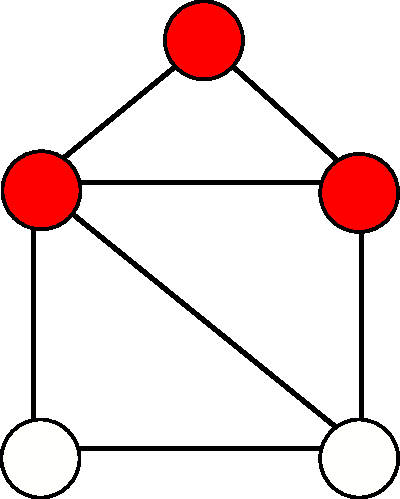
\includegraphics[height=30mm]{images/house_clique.pdf}
	\begin{block}{Definition}
		Eine \alert{$\ell$-Clique} in einem Graphen $G=(V,E)$ ist eine Menge $S\subseteq V$ von $|S|=\ell$ Knoten, so da\ss
		\begin{align*}
			uv\in E&&\mbox{f\"ur alle }u,v\in S,\,u\neq v.
		\end{align*}
		\itshape Mit anderen Worten: eine $\ell$-Clique ist eine Kopie von $K_\ell$ in $G$.
	\end{block}
\onslide<2>
		\hfill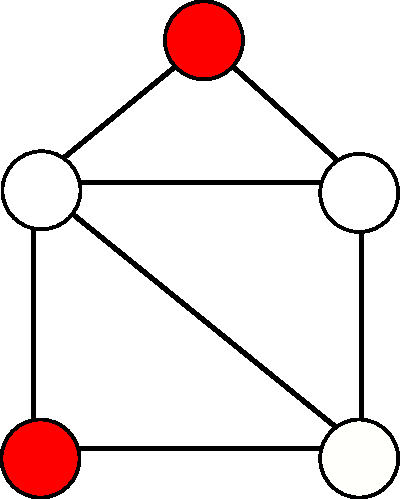
\includegraphics[height=30mm]{images/house_ind.pdf}
	\begin{block}{Definition}
		Eine \alert{$\ell$-stabile Menge} in einem Graphen $G=(V,E)$ ist eine Menge $S\subseteq V$ von $|S|=\ell$  Knoten, so da\ss
		\begin{align*}
			uv\not\in E&&\mbox{f\"ur alle }u,v\in S.
		\end{align*}
		\itshape Mit anderen Worten: eine $\ell$-stabile Menge ist eine Kopie von $\bar K_\ell$ in $G$.
	\end{block}
\onslide<3>
	\begin{block}{Definition}
		\begin{itemize}
			\item Die \alert{Cliquenzahl} von $G$ ist definiert als
				\begin{align*}
					\omega(G)=\max\cbc{S:S\mbox{ ist eine Clique in }G}.
				\end{align*}
			\item Die \alert{Stabilit\"atszahl} von $G$ ist definiert als
				\begin{align*}
					\alpha(G)=\max\cbc{S:S\mbox{ ist eine stabile Menge in }G}.
				\end{align*}
		\end{itemize}
	\end{block}
	\end{overprint}
\end{frame}

\begin{frame}\frametitle{\mytitle}
	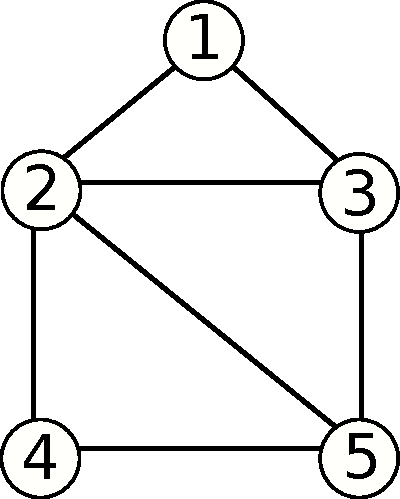
\includegraphics[height=30mm]{images/house.pdf}\hfill\parbox[t]{50mm}{\vspace{-26mm}$\bc{\begin{array}{ccccc}0&1&1&0&0\\1&0&1&1&1\\1&1&0&0&1\\0&1&0&0&1\\0&1&1&1&0\end{array}}$}
	\begin{overprint}
		\onslide<1>
		\begin{exampleblock}{Datenstruktur Adjazenzmatrix}
%			$G=(V,E)$ ist ein Graph mit $n=|V|$ Knoten und $m=|E|$ Kanten.
			\begin{itemize}
				\item die Adjazenzmatrix $A(G)$ ist ene $n\times n$-Matrix mit Eintr\"agen
					\begin{align*}
						A(G)_{uv}&=\vecone\cbc{uv\in E}&&(u,v\in V).
					\end{align*}
				\item die Zeilen/Spalten der Matrix sind durch die Knoten indiziert.
				\item die Matrix ist symmetrisch
			\end{itemize}
		\end{exampleblock}
		\onslide<2>
		\begin{exampleblock}{Datenstruktur Adjazenzmatrix}
			\begin{itemize}
				\item mittels der Adjazenzmatrix kann in $O(1)$ Zeit gepr\"uft, ob zwei Knoten benachbart sind
				\item alle Nachbarn eines Knoten zu finden, ben\"otigt $O(n)$ Zeit
				\item Speicherbedarf $\Theta(n^2)$
			\end{itemize}
		\end{exampleblock}
	\end{overprint}
\end{frame}

\begin{frame}\frametitle{\mytitle}
	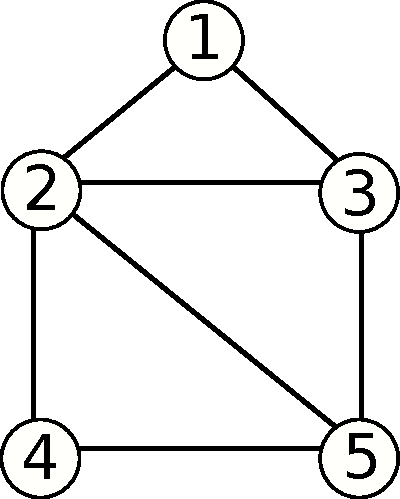
\includegraphics[height=30mm]{images/house.pdf}\hfill\parbox[t]{70mm}{\vspace{-26mm}$\begin{array}{cccccccccc}\alert{1}&\mapsto&2&\mapsto&3\\\alert{2}&\mapsto&1&\mapsto&3&\mapsto&4&\mapsto&5\\\alert{3}&\mapsto&1&\mapsto&2&\mapsto&5\\\alert{4}&\mapsto&2&\mapsto&5\\\alert5&\mapsto&2&\mapsto&3&\mapsto&4\end{array}$}
	\begin{overprint}
		\onslide<1>
		\begin{exampleblock}{Datenstruktur Adjazenzliste}
			\begin{itemize}
				\item jeder Knoten wird durch eine Liste repr\"asentiert
				\item die Liste enth\"alt seine Nachbarn
				\item die Reihenfolge ist beliebig
			\end{itemize}
		\end{exampleblock}
		\onslide<2>
		\begin{exampleblock}{Datenstruktur Adjazenzliste}
			\begin{itemize}
				\item Speicherbedarf $O(n+m)$
				\item um herauszufinden, ob $uv\in E$, ben\"otigen wir Zeit $O(\min\cbc{d_G(u),d_G(v)})$
				\item \emph{Sofern nicht anders angegeben, werden Graphen immer durch Adjazenzlisten dargestellt!}
			\end{itemize}
		\end{exampleblock}
	\end{overprint}
\end{frame}

\begin{frame}\frametitle{\mytitle}
	\begin{exampleblock}{Zusammenfassung}
		\begin{itemize}
			\item wir haben Grundbegriffe der Graphentheorie kennengelernt/wiederholt
			\item Adjazenzlisten sind eine geeignete Datenstruktur zur Darstellung von Graphen
		\end{itemize}
	\end{exampleblock}
\end{frame}
\end{document}
